\chapter{Giới thiệu}
\label{Chapter1}

%Tóm tắt luận văn được trình bày nhiều nhất trong 24 trang in trên hai mặt giấy, cỡ chữ Times New Roman 11 của hệ soạn thảo Winword hoặc phần mềm soạn thảo Latex đối với các chuyên ngành thuộc ngành Toán.

%Mật độ chữ bình thường, không được nén hoặc kéo dãn khoảng cách giữa các chữ.
%Chế độ dãn dòng là Exactly 17pt.
%Lề trên, lề dưới, lề trái, lề phải đều là 1.5 cm.
%Các bảng biểu trình bày theo chiều ngang khổ giấy thì đầu bảng là lề trái của trang.
%Tóm tắt luận án phải phản ảnh trung thực kết cấu, bố cục và nội dung của luận án, phải ghi đầy đủ toàn văn kết luận của luận án.
%Mẫu trình bày trang bìa của tóm tắt luận văn (phụ lục 1).

\section{Đặt vấn đề}
Ngôn ngữ là một loại phương tiện giúp con người có thể giao tiếp và truyền đạt suy nghĩ, ý kiến của mình cho những người xung quanh. Theo trang \textit{Ethnologue.com}\cite{Ethnologue}, tính đến năm 2022, trên thế giới có 7151 ngôn ngữ. Vì vậy, một người không thể nào học và hiểu hết mọi ngôn ngữ trên thế giới. Từ đó, có thế độ cần thiết của việc dịch từ một ngôn ngữ sang một ngôn ngữ khác. Ngành khoa học máy tính, cụ thể hơn là xử lý ngôn ngữ tự nhiên, chúng ta cũng tâm đến bài toán trên.

\begin{figure}[H]
    \begin{center}
        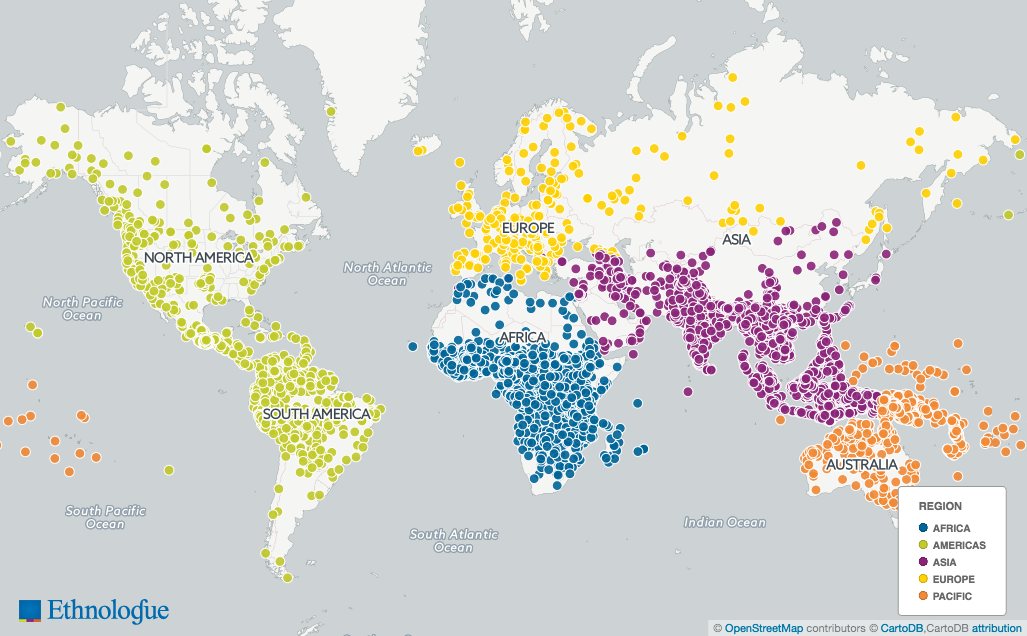
\includegraphics[scale=0.4]{images/number_of_langs}
        \caption{Phân bố các ngôn ngữ trên thế giới\cite{Ethnologue}}
        \label{fig:languages_distibuttion}
    \end{center}
\end{figure}

\section{Bài toán dịch máy (Machine Translation)}

Bài toán dịch máy là một lĩnh vực trong ngành khoa học máy tính. Đầu vào được nhập vào máy tính là một đoạn văn bản từ một ngôn ngữ (ngôn ngữ nguồn). Và qua quá trình xử lý, đưa ra được đoạn văn bản tương ứng ở một ngôn ngữ khác (ngôn ngữ đích). Khác với các mô hình xử lý ngôn ngữ khác, khi chúng chỉ cần một kho ngữ liệu của một ngôn ngữ. Các mô hình dịch máy cần ít nhất hai kho ngữ liệu của ngôn ngữ nguồn và ngôn ngữ đích. kho ngữ liệu bao gồm tập các đoạn văn bản. Với mỗi đoạn văn bản từ ngôn ngữ nguồn sẽ được ánh xạ đến một đoạn văn bản có ý nghĩa tương ứng ở ngôn ngữ đích. Các kho ngữ liệu này có thể tổng hợp từ các nguồn khác nhau: từ các bản dịch (subtitle) của các bộ phim, bản dịch sách và cả các bộ dữ liệu được thiết kế riêng cho bài toàn dịch máy (các bản dịch từ các chuyên gia).

Để có thể hiểu hơn sâu hơn bài toán và tìm ra hướng giải quyết, ta cần phải hiểu được cách tự nhiên mà con người dịch một đoạn văn bản từ ngôn ngữ nguồn sang ngôn ngữ đích như thế nào. Theo như \cite{2014arXiv1409.0473B}, quá trình này có thể chia làm hai bước:
\begin{itemize}
	\item Trích xuất ngữ cảnh, văn cảnh (\textit{context}) của ngôn ngữ nguồn thành thông tin.
	\item Chuyển hóa thông tin thu thập được thành ngôn ngữ đích.
\end{itemize}

\section{Các cách tiếp cận trước}

Với tính chất trên của bài toán, ta có thể thấy bài toán này là một bài toán \textit{sequence-to-sequence(Seq2Seq)} và có thể giải quyết bằng kiến trúc \textit{encoder-decoder}. Các mô hình sử dụng các mạng nơ ron hồi quy (Recursive Neural Network) sử dụng cơ chế Long-Short-Term-Memory.

\begin{figure}[H]
    \begin{center}
        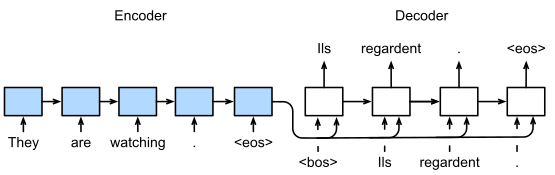
\includegraphics[scale=0.8]{images/seq2seq}
        \caption{Tổng quan kiến trúc mô hình Seq2Seq \cite{seq2seq}}
        \label{fig:seq2seq}
    \end{center}
\end{figure}


Các mô hình hồi quy (\textit{Recurrent model}) cho các các kết quả tốt trong bài toán dịch máy. Tuy nhiên, các mô hình này lại sử dụng cơ chế hồi quy. Ở mỗi bước tính toán, mô hình sử dụng thông tin ẩn (\textit{hidden state}) được tổng hợp từ đầu văn bản đến hiện tại $h_t$ để làm đầu vào tính toán. Quá trình này lặp lại cho mỗi bước. Từ đó, ta có thể thấy mô hình tính toán bước tiếp theo phải phụ thuộc vào bước trước đó, dẫn đến không thể song song quá trình tính toán này được. Điều này khiến cho việc tối ưu thời gian huấn luyện lẫn hiệu quả tính toán của mô hình trước nên khó khăn.

\begin{figure}[H]
    \begin{center}
        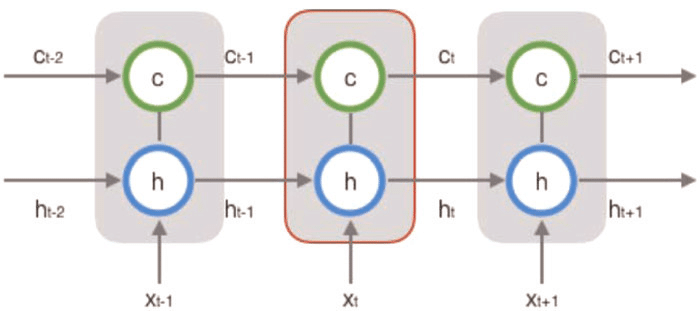
\includegraphics[scale=0.6]{images/hidden-state}
        \caption{Kiến trúc \textit{mạng hồi quy} với các thông tin ẩn}
        \label{fig:hidden state}
    \end{center}
\end{figure}

Một nhược điểm khác của các mô hình hồi quy đó là dễ xảy ra hiện tượng \textit{gradient biến mất} (\textit{Gradient Vanishing}) và đôi khi là \textit{gradient bùng nổ}(\textit{Gradient Exploding}). Nguyên nhân cốt lõi của vấn đề này là do công thức của hàm phi tuyến chưa hợp lý làm cho quá trình lan truyền ngược (\textit{back propagation}), các giá trị \textit{gradient} của mỗi lớp quá lớn hoặc quá nhỏ. Do đó làm cho \textit{gradient} lan truyền về sau trở nên càng lớn hoặc càng nhỏ theo cấp số mũ. Vấn đề \textit{gradient biến mất} sẽ làm cho mô hình hồi tụ chậm đi khi mô hình học sâu được tăng thêm số lớp. Để giải quyết vấn đề này, kiến trúc \textit{LSTM (long short term memory)} được giới thiệu. Với \textit{LSTM}, hiện tượng \textit{gradient biến mất} được cải thiện. Do đó khi mô hình đang xử lý ở bước thứ $i$, các thông tin từ các bước trước đó không bị mất đi. Nhờ vậy mà quá trình học ở bước hiện tại trở nên hiệu quả hơn.

\begin{figure}[H]
    \begin{center}
        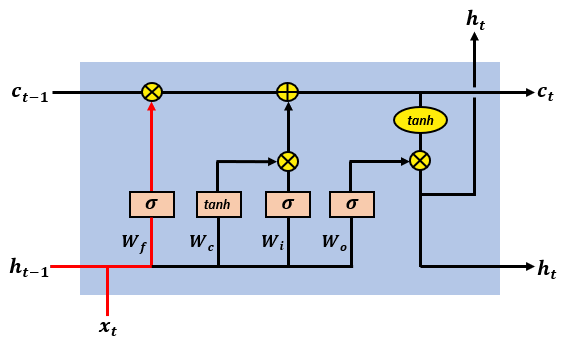
\includegraphics[scale=0.6]{images/lstm}
        \caption{Kiến trúc \textit{LSTM}}
        \label{fig:lstm}
    \end{center}
\end{figure}

\section{transformer}

\textit{transformer}\cite{transformer} - một phương pháp dựa hoàn toàn trên cơ chế attention, bỏ qua các cấu trúc của mạng nơ ron hồi quy và mạng nơ ron tích chập phức tạp, giúp đơn giản hóa mô hình những vẫn thể hiện được độ hiệu quả của mô hình. Theo \textbf{Paper attention is all your need} \cite{transformer}, mô hình cho kết quả 41.8 BLEU khi huấn luyện trên tập WMT 2014, cao hơn tất cả các mô hình dịch máy trước đó. 

\begin{figure}[H]
    \begin{center}
        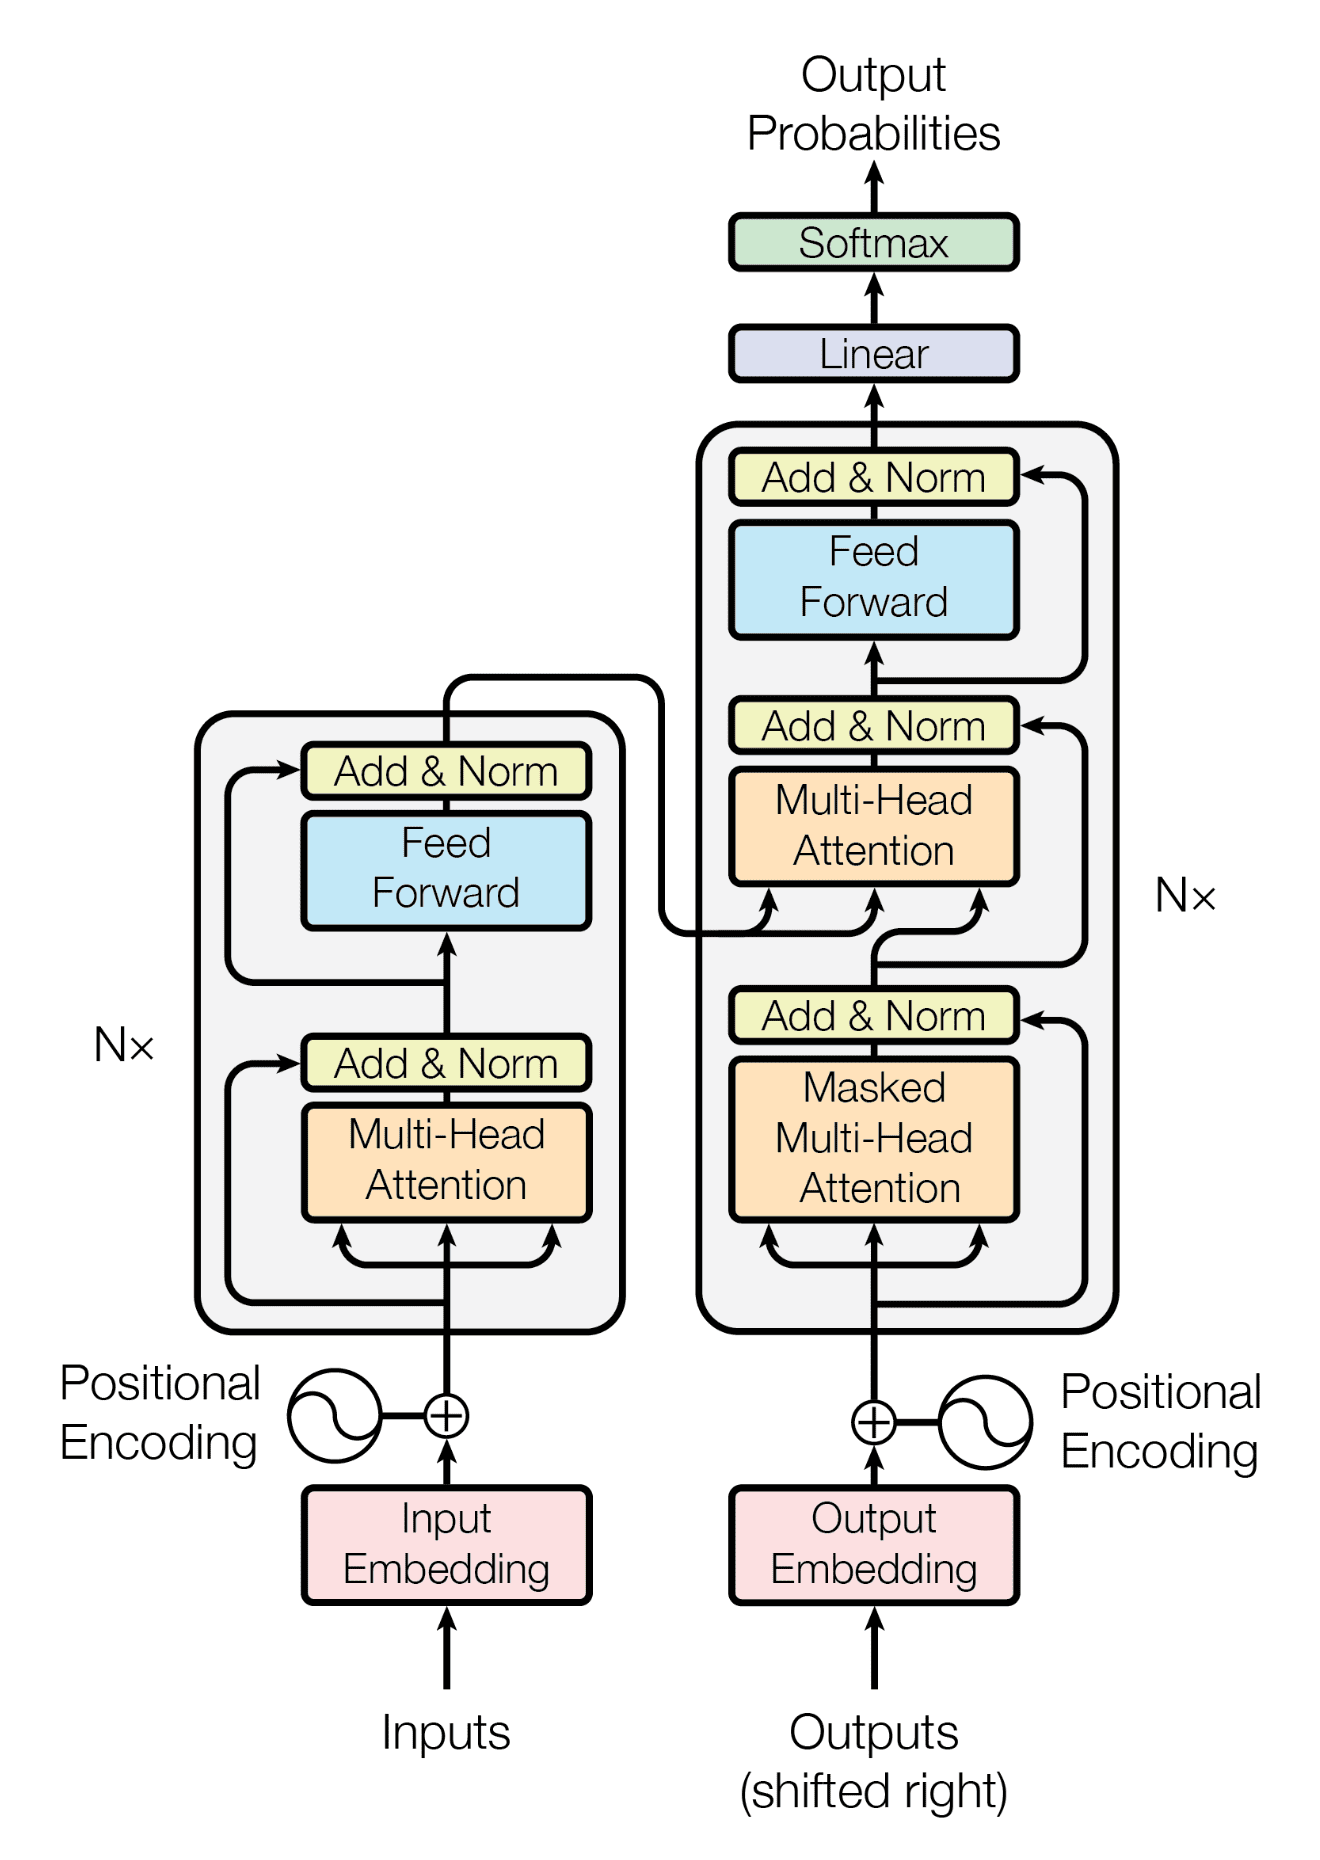
\includegraphics[scale=0.25]{images/attention-is-all-you-need}
        \caption{Tổng quan kiến trúc của \textit{ \textit{transformer} }}
        \label{fig:attetion-is-all-you-need}
    \end{center}
\end{figure}

Nhờ không sử dụng kiến trúc hồi quy, \textit{ \textit{transformer} } tránh được nhược điểm chí mạng của các mô hình loại này. Dựa hoàn toàn vào cơ chế \textit{attention}, cụ thể hơn là giới thiệu kiến trúc \textit{multihead-attention} giúp việc song song tính toán mô hình. Từ đó mà tăng độ hiệu quả huấn luyện cũng như hiệu quả tính toán.

\section{Tokenization \& Word Embeddings}

Trong bài toán dịch máy, các đoạn văn bản thô cần phải được tiền xử lý, chuyển đổi thành các dạng dữ liệu mà máy tính có thể hiểu được. Quá trình đó được thực hiện như sau:
\begin{itemize}
	\item \textit{Tokenization} là quá trình tách đoạn văn bản ra thành các từ thành phần (\textit{token}). Các token này đã được quy định sẵn trong một tập các từ đã biết trước được gọi là kho từ vựng (\textit{vocabulary}). Với các từ lạ, không thuộc trong kho từ vựng sẽ được đánh dấu là \textit{<unk> (unknown)}.
	\item Các \textit{token} sau khi được tách ra vẫn chưa thể đưa vào mô hình do chúng vẫn ở dạng dữ liệu mà các mô hình chưa thể hiểu. Do đó, với mỗi \textit{token}, ta cần chuyển chúng thành các vector N chiều (N chọn trước) mang tính chất và đại diện cho từ đó. Với mỗi chiều của vector được biểu diễn bằng một số thực. Các vector này được gọi là các \textit{Word Embeddings}. Các \textit{Word Embeddings} sẽ là đầu vào của mô hình. Một số phương pháp để tính toán các \textit{Word Embeddings} trước đây gồm: \textit{CBOW, N-gram, skip-gram,...}
\end{itemize}

\begin{figure}[H]
    \begin{center}
        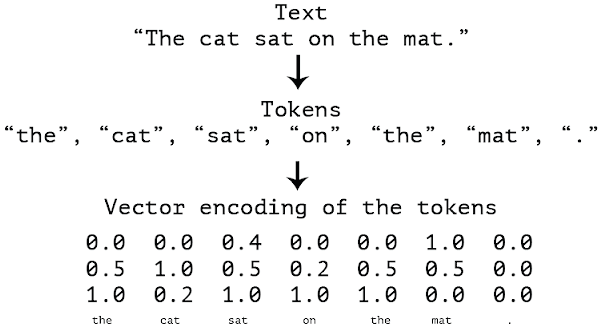
\includegraphics[scale=0.8]{images/token-embeddings}
        \caption{Tokenization \& word embeddings}
        \label{fig:\textit{SemGCN)}
    \end{center}
\end{figure}


\section{Graph Convolution Network (GCN)}
Khai thác quan hệ giữa các điểm dữ liệu với nhau là một đề tài được nhiều sự quan tâm trong học máy. Trong các mô hình học sâu trước đây, ta chỉ có thể trích xuất được các mối quan hệ thông thường từ các \textit{bộ dữ liệu Euclidian}.

\begin{figure}[H]
    \begin{center}
        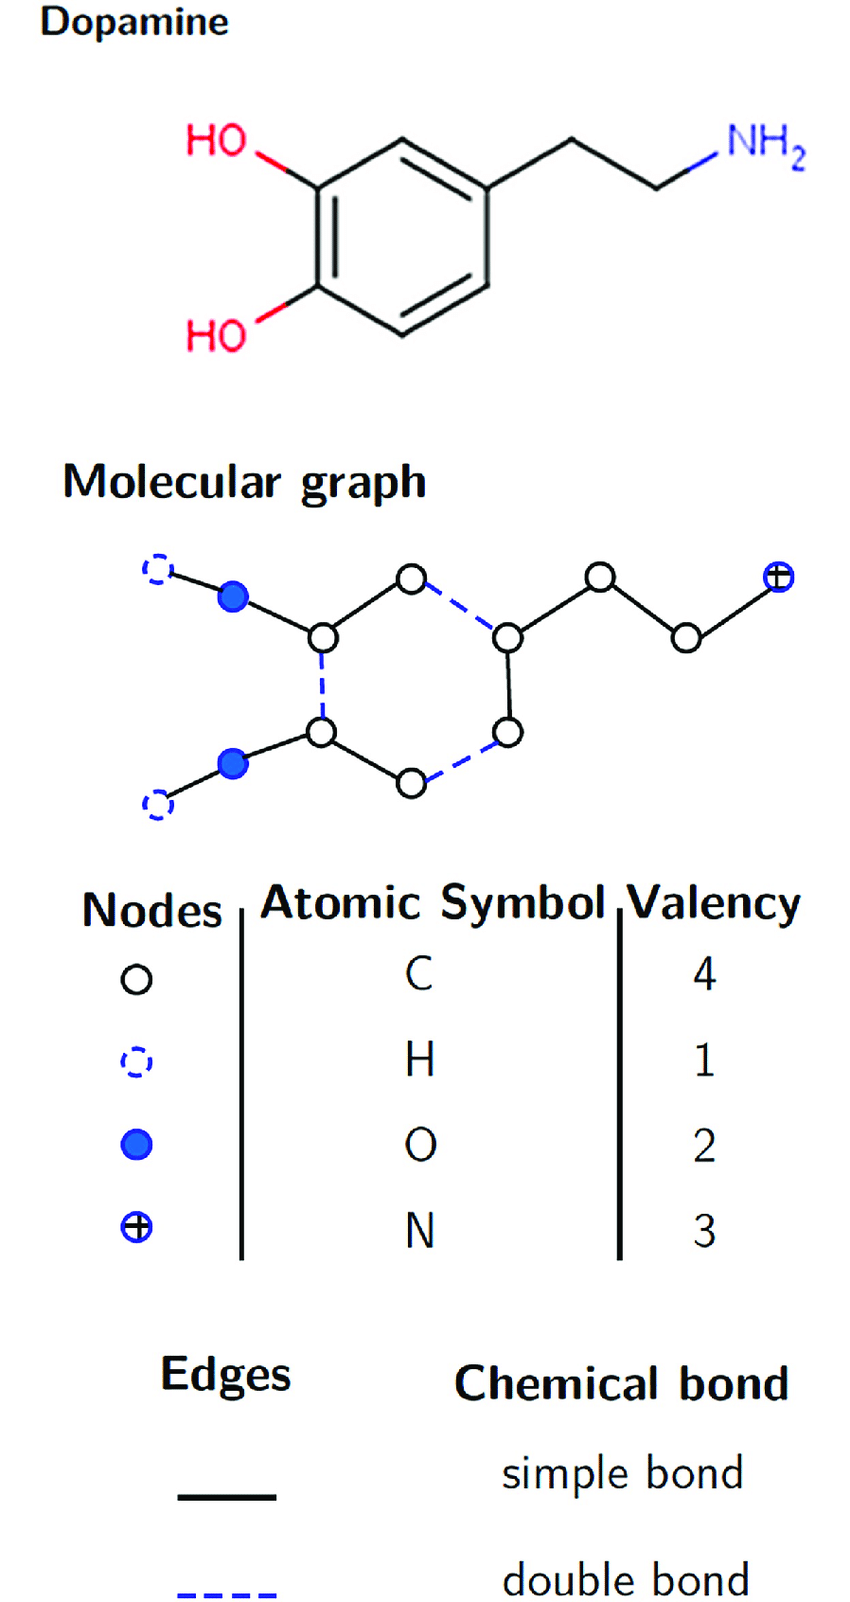
\includegraphics[scale=0.3]{images/chemistry-molecule}
        \caption{Các phân tử hóa học được biểu diễn dưới dạng đồ thị}
        \label{fig:chemistry-molecule}
    \end{center}
\end{figure}

Trong thực tế, không phải mọi dữ liệu đều biểu diễn ở dạng \textit{Euclidian}. Do đó, để khai thác được thông tin từ các bộ dữ liệu đồ thị (\textit{non-Euclidian}), ta cần sử dụng các mô hình \textit{Graph Neural Network (GNN)}. Trong vài năm qua, nhiều biến thể của đã được phát triển. Trong đó, \textit{Graph Convolution Network (GCN)} là một biến thể quan trọng được xem như là biến thể cơ bản nhất của \textit{Graph Neural Network(GNN)}.

\textit{Graph Convolutional Network} ứng dụng phép tích chập được giới thiệu trong \textit{convolution layer} của \textit{mạng tích chập(\textit{CNN})}:
\begin{itemize}
	\item Đối với phép tích chập trên \textit{\textit{CNN}}, một đoạn dữ liệu của lớp hiện tại sẽ được nhân vô hướng (tích chập) với một bộ lọc (\textit{filter} hoặc \textit{kernel}). Bộ lọc sẽ trượt trên bộ dữ liệu và các đầu ra của phép tích chập sẽ được truyền vào lớp tiếp theo của mạng.
	\item Với phép tích chập trên \textit{GCN}. Ta xét từng nút(\textit{node}) của đồ thị. Với mỗi nút, ta nhóm nút này với các nút kề của chính nó lại và thực hiền phép tích chập tương tự với một màn lọc. Do số lượng nút kề của mỗi nút là khác nhau, nên kích thước của \textit{filter} sẽ không cố định. Phép tích chập sẽ được thực hiện trên tất cả các nút của đồ thị.
\end{itemize}

\begin{figure}[H]
    \begin{center}
        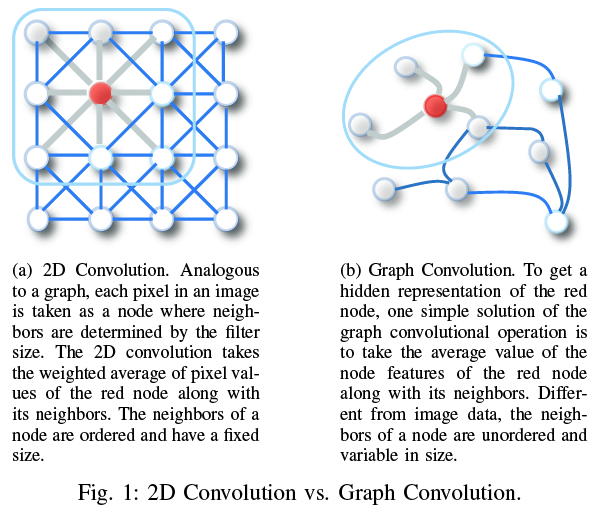
\includegraphics[scale=0.6]{images/cnn-vs-gcn}
        \caption{So sánh \textit{CNN} và \textit{GCN}}
        \label{fig:\textit{CNN}-vs-gcn}
    \end{center}
\end{figure}

Nhận xét về phép tích chập 2 chiều của mô hình \textit{CNN}. Nếu ta xem mỗi điểm dữ liệu là một đỉnh của đồ thị và các điểm dữ liệu xung quanh sẽ có cạnh nối đến với đỉnh tương ứng. Phép thích chập của \textit{CNN} có ý nghĩa hoàn toàn giống với phép tích chập của mô hình GCN.


\section{WordGCN}
Quan hệ của các từ trong một ngôn ngữ là dạng quan hệ non-Euclidian. Do đó, trích xuất thông tin của chúng bằng các mô hình \textit{GCN} được kì vọng là có kết quả tốt hơn các phương pháp trước đó. Các loại thông tin có thể khai thác bao gồm:
\begin{itemize}
	\item Thông tin về cú pháp (\textit{syntactic context}) của ngôn ngữ. Các từ trong một câu sẽ sẽ có các quy định về các mối quan hệ của chúng trong câu. Biểu diễn các mối quan hệ này là các cạnh còn các từ trong câu là các nút của đồ thị. Từ đó mà ta có thể khai thác được các đặc trưng cú pháp của các từ. Mô hình \textit{SynGCN} sẽ giúp ta huấn luyện được các embeddings mang các thông tin trên

    \begin{figure}[H]
        \begin{center}
            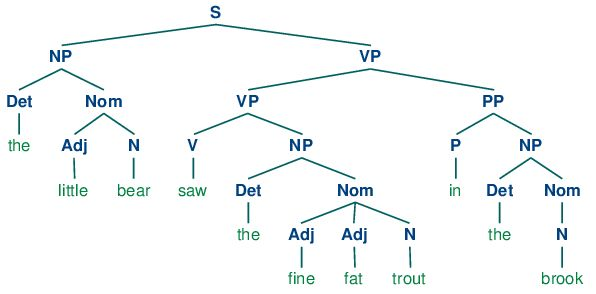
\includegraphics[scale=0.8]{images/syntactic-context}
            \caption{Thông tin cú pháp của một câu được biểu diễn dưới dạng đồ thị}
            \label{fig:syntactic-context}
        \end{center}
    \end{figure}

	\item Thông tin về ngữ nghĩa (\textit{semantic}) của ngôn ngữ. Ý nghĩa của các từ sẽ có các quan hệ với nhau như: đồng nghĩa, trái nghĩa, kế thừa,... Nhờ các mối quan hệ đó, ta có thể biểu diễn được đồ thị ngữ nghĩa của các từ trong bộ từ vựng. Từ đó mà ta có thể khai thác được các đặc trưng ngữ nghĩa của các từ. Mô hình \textit{\textit{SemGCN)} sẽ giúp ta huấn luyện được các \textit{embeddings} mang thông tin ngữ nghĩa.

    \begin{figure}[H]
        \begin{center}
            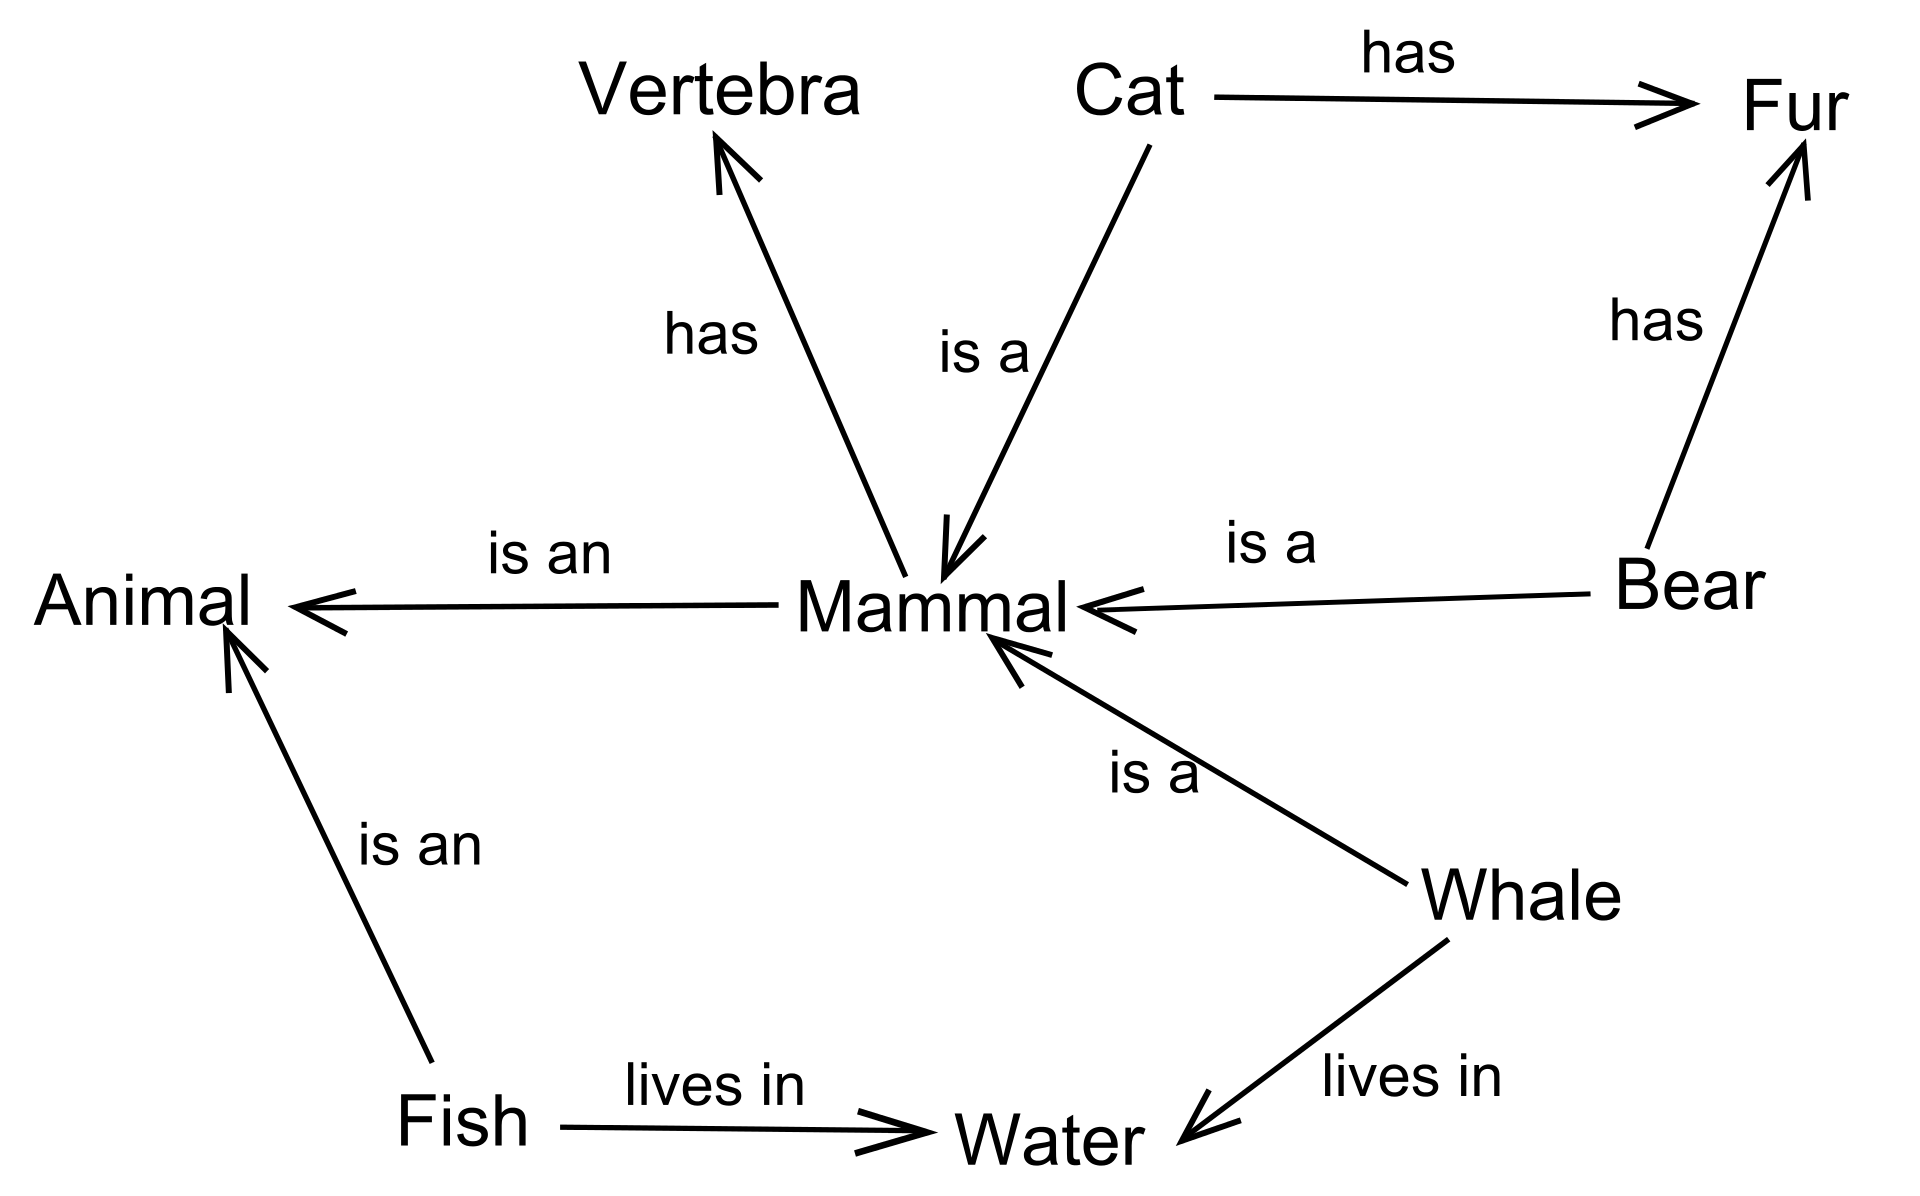
\includegraphics[scale=0.2]{images/semantic-context}
            \caption{Thông tin ngữ nghĩa của các từ được biểu diễn dưới dạng đồ thị}
            \label{fig:semantic-context}
        \end{center}
    \end{figure}

\end{itemize}